\UseRawInputEncoding
%%%%%%%%%%%%%%%%%%%%%%%%%%%%%%%%%%%%%%%%%%%%%%%%%%%%%%%%%%%%%%%%%%%%%%%%%%%%%%%%%%%%%%%%%%%%%%%%%%%%%%%
%%%%%%%%%%%%%% Template de Artigo Adaptado para Trabalho de Conclusão de Curso - SI Contagem - PUCMINAS %%%%%%%%%%%%%%%%%%%%%%%%
%% codificação UTF-8 - Abntex - Latex -  							     %%
%% Autor da primeira versão:    Fábio Leandro Rodrigues Cordeiro  (fabioleandro@pucminas.br)                            %% 
%% Co-autor da primeira versão: Prof. João Paulo Domingos Silva, Harison da Silva e Anderson Carvalho                   %%
%% Revisores normas NBR (Padrão PUC Minas) da primeira versão: Helenice Rego Cunha e Prof. Theldo Cruz                  %%
%% Versão: 1.1     18 de dezembro 2015                     	                                     %%
%%%%%%%%%%%%%%%%%%%%%%%%%%%%%%%%%%%%%%%%%%%%%%%%%%%%%%%%%%%%%%%%%%%%%%%%%%%%%%%%%%%%%%%%%%%%%%%%%%%%%%%


\documentclass[a4paper,12pt]{article}
\usepackage[utf8]{inputenc}
\usepackage{times}
\usepackage{abakos}  %pacote com padrão da Abakos baseado no padrão da PUC
%%%%%%%%%%%%%%%%%%%%%%%%%%%
%Capa da revista
%%%%%%%%%%%%%%%%%%%%%%%%%%

%\setcounter{page}{80} %iniciar contador de pagina de valor especificado
\newcommand{\monog}{Desenvolvimento de uma Aplicação com base na IA Gemini para Analisar e Identificar Novos Pontos Comerciais de Lojas: estudo de caso de expansão do Starbucks\texttrademark}

%\newcommand{\monogES}{Article template Institute of Mathematical Sciences and Informatics}
\newcommand{\tipo}{Artigo}  % Especificar a seção tipo do trabalho: Artigo, Resumo, Tese, Dociê etc
%\newcommand{\origem}{Brasil}
%\newcommand{\editorial}{Belo Horizonte, p. 01-11, nov. 2024}  % p. xx-xx – páginas inicial-final do artigo
\newcommand{\editorial}{}  
\newcommand{\lcc}{\scriptsize{Licença Creative Commons Attribution-NonCommercial-NoDerivs 3.0 Unported}}

%%%%%%%%%%%%%%%%%INFORMAÇÕES SOBRE AUTOR PRINCIPAL %%%%%%%%%%%%%%%%%%%%%%%%%%%%%%%
\newcommand{\AutorA}{Andressa Assunção Nunes}
\newcommand{\funcaoA}{Aluna }

\newcommand{\emailA}{\href{mailto:xxx@sga.pucminas.br}{1334884@sga.pucminas.br}}
\newcommand{\cursA}{do Programa de Graduação em Sistemas de Informação}

\newcommand{\AutorC}{Wesley Dias Maciel}
\newcommand{\funcaoC}{}
\newcommand{\emailC}{\href{mailto:xxx@sga.pucminas.br}{45520@sga.pucminas.br}}
\newcommand{\cursC}{Professor(a) do Programa de Graduação em Sistemas de Informação}
% 
% Definir macros para o nome da Instituição, da Faculdade, etc.
\newcommand{\univ}{Pontifícia Universidade Católica de Minas Gerais}

\newcommand{\keyword}[1]{\textsf{#1}}

%Para as URLS não ultrapassarem a margem
\usepackage{url}
\makeatletter
\g@addto@macro{\UrlBreaks}{\UrlOrds}
\makeatother

\usepackage{adjustbox} % reduzir tamanho figuras

\usetikzlibrary{arrows,shapes,positioning,shadows,trees}

\tikzset{
  basic/.style  = {draw, text width=3cm, drop shadow, font=\sffamily, rectangle},
  root/.style   = {basic, rounded corners=2pt, thin, align=center,
                   fill=blue!30},
  level 2/.style = {basic, rounded corners=6pt, thin,align=center, fill=green!30,
                   text width=8em},
  level 3/.style = {basic, thin, align=left, fill=pink!60, text width=6.5em}
}

\usepackage{listings}
\usepackage{xcolor}

% Definindo as cores do Dark Mode
\definecolor{fundoEscuro}{HTML}{1E1E1E}
\definecolor{textoClaro}{HTML}{D4D4D4}
\definecolor{palavraChave}{HTML}{569CD6}
\definecolor{textoString}{HTML}{CE9178}

\lstset{
    backgroundcolor=\color{fundoEscuro},
    basicstyle=\ttfamily\color{textoClaro}\footnotesize,
    keywordstyle=\color{palavraChave}\bfseries,
    stringstyle=\color{textoString},
    breakatwhitespace=false,         
    breaklines=true,                 
    captionpos=b,                    
    keepspaces=true,                 
    numbers=none,                    
    showspaces=false,                
    showstringspaces=false,
    showtabs=false,                  
    tabsize=4,
    extendedchars=true,
    literate={á}{{\'a}}1 {ã}{{\~a}}1 {é}{{\'e}}1 {ó}{{\'o}}1 {í}{{\'i}}1 {ç}{{\'c}}1 {õ}{{\~o}}1 % Para lidar com acentos em PT-BR
}

\usepackage{caption}
\usepackage{listings}

% Muda o nome de "Listing" para "Algoritmo"
\renewcommand{\lstlistingname}{Algoritmo}

% Deixa "Algoritmo X:" em negrito, o texto normal, e alinhado à esquerda
\captionsetup[lstlisting]{labelfont=bf, textfont=normalfont, labelsep=colon, justification=raggedright, singlelinecheck=false}

% \usepackage{caption}
% \captionsetup[quadro]{labelfont=bf, labelsep=colon, justification=raggedright, singlelinecheck=false}

\usepackage{hyperref}

\begin{document}
% %%%%%%%%%%%%%%%%%%%%%%%%%%%%%%%%%%
% %% Pagina de titulo
% %%%%%%%%%%%%%%%%%%%%%%%%%%%%%%%%%%
\citeoption{abnt-doi=link}
\citeoption{abnt-url-package=url}

\begin{center}

\includegraphics[scale=0.2]{figuras/brasao.jpg} \\
PONTIFÍCIA UNIVERSIDADE CATÓLICA DE MINAS GERAIS \\
Instituto de Ciências Exatas e de Informática

% \vspace{1.0cm}

\end{center}

 \vspace{0cm} {
 \singlespacing \Large{\monog \symbolfootnote[1]{Artigo apresentado ao Instituto de Ciências Exatas e Informática da Pontifícia Universidade Católica de \linebreak Minas Gerais, campus Contagem, como pré-requisito parcial para obtenção do título de Bacharel em Sistemas de Informação.} \\ }
 % \normalsize{\monogES}
 }

\vspace{1.0cm}

\begin{flushright}
\singlespacing 
\normalsize{\AutorA \footnote{\funcaoA \cursA \,-- \emailA . }} \\
\normalsize{\AutorC \footnote{\funcaoC \cursC \,-- \emailC . }} \\
%\normalsize{\AutorD \footnote{\funcaD \cursD \,-- \emailD . }} \\
\end{flushright}
\thispagestyle{empty}

\vspace{1.0cm}

\begin{abstract}
\noindent
A expansão física de varejos de grande escala exige o processamento de volumes massivos de dados espaciais e socioeconômicos para embasar decisões estratégicas. Contudo, os modelos analíticos tradicionais apresentam subjetividade e carência de ferramentas para a simulação de cenários personalizados. Diante dessa lacuna, torna-se necessário integrar soluções tecnológicas que reduzam a incerteza na escolha de novos pontos comerciais. O objetivo deste trabalho foi desenvolver e avaliar uma plataforma baseada em Inteligência Artificial para a identificação de vazios comerciais e suporte à decisão em \textit{Business Intelligence} (BI). Metodologicamente, a pesquisa foi caracterizada como aplicada e quantitativa, adotando o formato de estudo de caso com dados geográficos da rede Starbucks\texttrademark referentes ao ano de 2023, processados na linguagem Python e integrados com a API do modelo Gemini. Os resultados demonstraram que o sistema delimita as regiões mais promissoras por meio de zonas de intensidade, gerando relatórios a partir de indicadores de renda, densidade demográfica, fluxo de pedestres e perfil do público. A conclusão do trabalho foi que a ferramenta contribuiu para mitigar riscos na criação de novas lojas, oferecendo uma metodologia escalável que garante a sustentabilidade da expansão organizacional no mercado físico.
\\\textbf{\keyword{Palavras-chave:}} Inteligência Artificial. Vazios Comerciais. Expansão Varejista. \textit{Business Intelligence}.
\end{abstract}

%%%%%%%%%%%%%%%%%%%%%%%%%%%%%%%%%%%%%%%%%%%%%%%%%%%%%%%%%
\selectlanguage{english}
\begin{abstract}
\noindent
The physical expansion of large-scale retail requires the processing of massive volumes of spatial and socioeconomic data to support strategic decisions. However, traditional analytical models present subjectivity and a lack of modular tools for simulating customized scenarios. Given this gap, it is essential to integrate technological solutions that reduce uncertainty in the selection of new commercial locations. This study aims to develop and evaluate an interactive Artificial Intelligence-based platform for identifying commercial voids and supporting decision-making in Business Intelligence (BI). Methodologically, the research is characterized as applied and quantitative, adopting a case study approach with 2023 geographic data from the Starbucks chain, processed using the Python language and integrated with the Gemini model API. The results demonstrate that the developed interface delimits the most promising regions through intensity zones, generating automated reports based on indicators of income, population density, pedestrian flow, and audience profile. It is concluded that the tool significantly contributes to mitigating risks in the viability of new stores, offering a scalable methodology that ensures the sustainability of organizational expansion in the physical market.
\\\textbf{\keyword{Keywords:}} artificial intelligence; commercial voids; retail expansion; business intelligence; Starbucks.
\end{abstract}

\selectlanguage{brazilian}
 \onehalfspace  % espaçamento 1.5 entre linhas
 \setlength{\parindent}{1.25cm}

%%%%%%%%%%%%%%%%%%%%%%%%%%%%%%%%%%%%%%%%%%%%%%%%%
%% INICIO DO TEXTO
%%%%%%%%%%%%%%%%%%%%%%%%%%%%%%%%%%%%%%%%%%%%%%%%%

%%%%%%%%%%%%%%%%%%%%%%%%%%%%%%%%%%%%%%%%%%%%%%%%%%%%%%%%%%%%%%%%%%%%%%%%%%%%%%%%%%%%%%%%%%%%%%%%%%%%%%%%%%%%%%%%%%%%%%%%%%%%%%%%
%%%%%%%%%%%%%% Template de Artigo Adaptado para Trabalho de Conclusão de Curso - SI Contagem - PUCMINAS                       %%
%% codificação UTF-8 - Abntex - Latex -  							                                                          %%
%% Autor da primeira versão:    Fábio Leandro Rodrigues Cordeiro                                                              %% 
%% Co-autores da primeira versão: Prof. João Paulo Domingos Silva, Harison da Silva e Anderson Carvalho		                  %%
%% Revisores normas NBR (Padrão PUC Minas) da primeira versão: Helenice Rego Cunha e Prof. Theldo Cruz                        %%
%% Versão: 1.1     18 de dezembro 2015                                                                                        %%
%%%%%%%%%%%%%%%%%%%%%%%%%%%%%%%%%%%%%%%%%%%%%%%%%%%%%%%%%%%%%%%%%%%%%%%%%%%%%%%%%%%%%%%%%%%%%%
\section{\esp Introdução}

A expansão física de varejos de grande escala exige o processamento de volumes massivos de dados para tomadas de decisão informadas \cite{mallela2024}. No contexto de redes como a Starbucks, que mantém mais de 25 mil unidades distribuídas em 73 países, a abertura de um único ponto comercial em uma região inadequada pode representar um prejuízo operacional da ordem de centenas de milhares de dólares em arrendamento, obras e treinamento de pessoal, sem contar o custo de oportunidade de não ter escolhido uma localização melhor. Decisões dessa magnitude não podem depender da intuição ou da experiência individual de um analista. Modelos analíticos tradicionais apresentam performance sujeita à subjetividade do \textit{designer}, o que compromete a precisão estratégica e a visibilidade sobre o mercado físico \cite{mallela2024, okorie2024}. A literatura carece, ainda, de ferramentas que permitam simular cenários customizados em diferentes segmentações de mercado \cite{rajan2024}. Esta pesquisa investiga de que maneira uma solução de Inteligência Artificial (IA) auxilia na análise estratégica de expansão. Utilizamos a rede Starbucks como cenário de validação.

Este trabalho desenvolveu a plataforma \textit{Retail Insights} (disponível em: \url{https://retail-expansion.streamlit.app/}) para identificação de novos pontos comerciais e suporte à decisão em \textit{Business Intelligence} (BI). A solução permite que o usuário crie cenários prospectivos por meio de variáveis como renda da população, densidade demográfica e fluxo de pedestres. Para demonstrar sua funcionalidade, utilizamos dados históricos de 2023 da rede Starbucks, disponibilizados na plataforma \href{https://www.kaggle.com/datasets/omarsobhy14/starbucks-store-location-2023}{Kaggle} \cite{omarsobhy2023}. O sistema mapeou a distribuição geográfica atual e gerou análises técnicas para identificação de novos pontos. A ferramenta implementou \textit{Key Performance Indicators} (KPIs) automatizados, baseados em regras de negócio e geolocalização, detalhando indicadores de renda, densidade demográfica e perfil do público.

Como principal resultado, a ferramenta delimita as regiões mais promissoras por meio de zonas de intensidade. A interface permite diagnosticar problemas operacionais e identificar relações de causa e efeito entre variáveis geográficas em diversos contextos de varejo. Esta pesquisa contribui para a redução da incerteza na viabilidade de pontos comerciais e oferece uma metodologia escalável que sustenta a expansão organizacional no mercado físico \cite{dahake2024}.


\section{\esp Referencial Teórico}

O conceito de \textit{Business Intelligence} (BI) surgiu em 1865. Richard Millar Devens descreveu estratégias para decisões fundamentadas no histórico de dados e conhecimento de mercado \cite{dama2009}. Em 1958, Hans Peter Luhn propôs sistemas automáticos para extrair e codificar dados para disseminar informações \cite{luhn1958}. A ciência de dados classifica dados brutos como estruturados, semiestruturados ou não estruturados \cite{sharda2019}. Atualmente, a transição para a era de \textit{Data \& Insights} exige que as organizações vão além da simples coleta. A integração de soluções de Inteligência Artificial (IA) converte métricas operacionais em Indicadores-Chave de Desempenho (KPIs). Esse processo permite monitorar o retorno sobre investimento por meio de interfaces interativas \cite{laudon2014}.

\subsection{\esp Business Intelligence e Data \& Insights} \label{subsec:bi_data}
O \textit{Business Intelligence} (BI) moderno combina arquiteturas, ferramentas e metodologias para transformar dados brutos em informações estratégicas \cite{sharda2019, barbieri2020}. A era de \textit{Data \& Insights} fundamenta-se no processo de datificação. Nesse contexto, registros temporais e interações sociais deixam de ser silos isolados. Eles compõem uma memória organizacional estratégica \cite{barbieri2020}. Para essa transformação, é imperativo usar repositórios integrados, como o \textit{Data Warehouse} (DW). O DW permite explorar variáveis por meio de técnicas de pré-processamento e limpeza de dados \cite{sharda2019, dama2009}. No cenário corporativo, essa estrutura possibilita que dados de geolocalização gerem \textit{insights} sobre a viabilidade de novos pontos comerciais.

\subsection{\esp Business Intelligence e Cultura Data-Driven} \label{subsec:bi_datadriven}
O \textit{Business Intelligence} (BI) moderno evoluiu para a cultura \textit{data-driven}, na qual a tomada de decisão estratégica é fundamentada em evidências empíricas e análises objetivas de fatos, em detrimento da intuição \cite{sharda2019}. Os princípios dessa abordagem compreendem: (i) coleta rigorosa de dados de múltiplas fontes internas e externas; (ii) processamento contínuo, preferencialmente em tempo real, por meio de \textit{pipelines} automatizados; (iii) conversão de métricas brutas em \textit{insights} acionáveis; e (iv) disseminação da informação por toda a organização, de modo que cada decisão seja rastreável e justificável \cite{barbieri2020}.

Sua relevância para este trabalho é direta: a cultura \textit{data-driven} substitui o julgamento subjetivo do analista de expansão por um conjunto mensurável de indicadores socioeconômicos e geográficos. No varejo, essa postura permite identificar padrões de consumo invisíveis a olho nu -- como correlações entre fluxo de pedestres, renda familiar e saturação comercial. A expansão geográfica, assim, responde a demandas reais e mensuráveis de mercado, em vez de avaliações pontuais baseadas em experiência individual.

\subsection{\esp Inteligência Artificial como Suporte à Decisão} \label{subsec:ia_decisao}
A IA funciona como um motor essencial para superar as limitações cognitivas humanas no processamento de volumes massivos de dados \cite{sharda2019}. Ao integrar algoritmos de \textit{Machine Learning} a sistemas transacionais, as organizações realizam análises preditivas precisas \cite{dahake2024, rajan2024}. \citeonline{dahake2024} demonstrou que a fusão de IA e análise de dados transforma as estratégias de \textit{marketing}. Essa sinergia promove uma abordagem \textit{data-driven}, na qual a IA interpreta oscilações em tempo real. Consequentemente, a liderança toma decisões táticas fundamentadas em evidências. Tal prática minimiza a subjetividade inerente ao processo decisório \cite{rajan2024, peri2025}. Para a expansão varejista, esse suporte diagnostica relações entre o fluxo de pedestres e a rentabilidade esperada.
\subsection{\esp Algoritmos de Boosting e IA no Varejo} \label{subsec:algoritmos}
A literatura aponta que algoritmos de \textit{Ensemble Learning} — métodos que combinam múltiplos modelos fracos para formar um preditor robusto — são os mais eficazes para a análise de localização. O \textit{AdaBoost} (Adaptive Boosting) funciona em ciclos iterativos: a cada rodada, ele instancia um classificador fraco (geralmente uma árvore de decisão rasa), mede os acertos e erros e repondera as amostras, atribuindo maior peso aos registros classificados incorretamente. Ao final do processo, os classificadores fracos recebem um peso proporcional à sua acurácia e são combinados por voto majoritário, resultando em um modelo final que corrige sistematicamente os erros das iterações anteriores \cite{peri2025}. No contexto varejista, essa propriedade é útil para segmentar perfis de consumidores e identificar quais combinações de variáveis socioeconômicas diferenciam regiões de alta potencial das demais.

Já o \textit{Gradient Boosting} adota princípio análogo, porém otimiza uma função de perda diferenciável por meio do gradiente descendente: cada novo modelo ajusta-se ao \textit{resíduo} (erro) deixado pelo conjunto anterior, reduzindo progressivamente o erro em direção ao mínimo global. Essa característica permite prever o sucesso de um ponto comercial com alta granularidade, pois modelos baseados em gradiente conseguem capturar relações não lineares entre renda, densidade demográfica e fluxo de pedestres, variáveis que tipicamente definem o desempenho de uma loja \cite{nair2022}. A escolha dessa família de algoritmos justifica-se pela superioridade empírica demonstrada em tarefas tabulares com dados heterogêneos, exatamente o perfil dos cadastros de expansão varejista.

A aplicação de \textit{Internet of Things} (IoT) complementa esses modelos. IoT refere-se à rede de objetos físicos equipados com sensores, software e conectividade que trocam dados pela internet sem intervenção humana direta — exemplos cotidianos incluem câmeras de contagem de pessoas, sensores de tráfego veicular, lixeiras inteligentes e dispositivos de pagamento. Ao fornecer variáveis dinâmicas de tráfego de pedestres em tempo real — dados que modelos estáticos baseados apenas em censos demográficos não conseguem captar —, a IoT abre espaço para que algoritmos de \textit{boosting} incorporam uma dimensão temporal à análise de localização, aumentando a assertividade das previsões \cite{leung2020, wang2024}.


\subsection{\esp Inteligência Artificial na Expansão do Varejo} \label{subsec:ia_varejo}
A IA na análise de expansão varejista utiliza modelos preditivos para otimizar a escolha de localizações físicas. O processo integra dados de geolocalização e variáveis socioeconômicas \cite{rajan2024, okorie2024}. Técnicas como o algoritmo \textit{AdaBoost} constroem modelos robustos que identificam potenciais de mercado inexplorados \cite{peri2025, mallela2024}. Em varejos de grande escala, modelos de IA e \textit{Big Data} preveem a demanda e automatizam a gestão de inventários \cite{leung2020}. \citeonline{wang2024} propôs um \textit{framework} baseado em \href{https://www.ibm.com/topics/internet-of-things}{\textit{IoT}} e otimização para aumentar a eficiência da cadeia de suprimentos.

Contudo, a literatura aponta que implementar esses modelos no ambiente físico enfrenta desafios. Um exemplo é a visibilidade limitada do comportamento \textit{in-store} \cite{malvankar2023, okorie2024}. O sucesso da expansão organizacional depende de \textit{frameworks} de \textit{design} que facilitem a visualização de resultados complexos. Interfaces baseadas em \textit{dashboards} e mapas de alta granularidade cumprem esse papel \cite{sharda2019}. Assim, a interface desenvolvida para o caso Starbucks executa a leitura do arquivo e projeta cenários. A ferramenta permite identificar novos pontos comerciais definidos por coordenadas geográficas precisas.

\section{\esp Trabalhos Relacionados}

\citeonline{liu2025} investigaram a viabilidade estratégica de novas unidades físicas. Eles propuseram um modelo de jogo evolutivo tripartido para analisar microdepósitos farmacêuticos não tripulados. O estudo focou na disposição estratégica de empresas, fornecedores e consumidores. Para isso, os autores utilizaram simulações numéricas para verificar a estabilidade do equilíbrio na implementação de novos pontos de venda. As semelhanças com esta pesquisa residem no foco central na tomada de decisão para expansão física. Entretanto, enquanto \citeonline{liu2025} utilizaram a Teoria dos Jogos para modelar o comportamento de \textit{stakeholders}, este trabalho propõe uma interface baseada em IA. Utilizamos dados geográficos e KPIs de densidade populacional para identificar novos pontos comerciais de forma visual. Tal abordagem permite que a rede Starbucks visualize áreas de expansão com critérios técnicos objetivos.

A pesquisa de \citeonline{oldemeyer2024} enfatizou a importância da IA para a evolução da estratégia corporativa. Os autores destacaram os desafios de implementação no cenário das pequenas e médias empresas. Contudo, este trabalho diferencia-se ao transitar da análise teórica para o desenvolvimento prático. Desenvolvemos uma ferramenta aplicada ao estudo de caso da rede Starbucks. A solução oferece alta granularidade analítica baseada em coordenadas de latitude e longitude. Dessa forma, mitigamos a incerteza decisória apontada pela autora.

Por fim, \citeonline{nair2022} exploraram a Inteligência Artificial embarcada na indústria varejista. O estudo focou na otimização do \textit{design} de produtos e no planejamento de lojas por meio de algoritmos como o \textit{Gradient Boost}. O trabalho demonstrou como a IA aumenta a precisão na análise da estrutura de intensidade e produtividade comercial. A semelhança com esta pesquisa está no emprego de algoritmos de aprendizado de máquina para elevar a precisão analítica no varejo moderno. A diferença fundamental reside no escopo. Enquanto \citeonline{nair2022} focaram na organização interna e no \textit{design} do item, esta pesquisa direciona a IA para a análise de expansão externa. Nossa ferramenta utiliza círculos de potencial geográfico e zonas de vazio comercial. Esses elementos orientam a liderança estratégica na escolha de novos pontos de presença física.

\section{\esp Desenvolvimento}

O desenvolvimento da plataforma \textit{Retail Insights} criou um sistema de suporte à identificação de novos pontos comerciais. Esta seção detalha o ambiente experimental, o modelo lógico da ferramenta e a implementação técnica do \textit{software}.

\subsection{\esp Ambiente de Desenvolvimento e Arquitetura}

Estruturamos o ambiente na linguagem Python para garantir a integridade e a portabilidade do sistema. A arquitetura do projeto compõe-se de três elementos fundamentais:

\begin{itemize}
    \item \textbf{Ambiente Virtual (\texttt{.venv}):} Isola as dependências. Garante que as bibliotecas \textit{Streamlit, Pandas, Folium} e \textit{Supabase} operem em versões controladas, sem interferência do interpretador global.
    \item \textbf{Controle de Versão (\texttt{.gitignore}):} Omite a pasta \texttt{.venv}, arquivos de cache (\texttt{\_\_pycache\_\_}) e credenciais sensíveis (\texttt{.streamlit/secrets.toml}). Segue as boas práticas de segurança no desenvolvimento de \textit{software}.
    \item \textbf{Script Principal (\texttt{retail-expansion-ai.py}):} Integra a lógica da interface, o processamento de dados, a comunicação com a \textit{API} de Inteligência Artificial e o banco de dados em nuvem \textit{Supabase}.
    \item \textbf{Pacote \texttt{fallback/}:} Módulo Python que contém dicionários de dados \textit{offline} (ex.: \texttt{store\_images.py}), garantindo resiliência quando o banco de dados está indisponível.
    \item \textbf{Banco de Dados em Nuvem (\textit{Supabase}):} Hospeda as tabelas \texttt{lojas} (CSV migrado), \texttt{respostas} (avaliações \textit{Likert}) e \texttt{store\_images} (referências arquitetônicas categorizadas). Todas as tabelas possuem \textit{Row Level Security} (RLS) habilitada.
\end{itemize}

\subsection{\esp Modelo Lógico da Ferramenta}

Definimos o modelo lógico para atender às necessidades de um Analista de Expansão. A ferramenta permite a transição entre a análise de dados históricos e a prospecção preditiva.

\subsubsection{\esp Requisitos do Sistema}

Levantamos os requisitos funcionais (RF) e não funcionais (RNF) essenciais para a viabilidade da ferramenta:

\begin{itemize}
    \item \textbf{RF01 - Ingestão de Dados:} O sistema deve processar coordenadas geográficas e metadados corporativos a partir do banco \textit{Supabase} (tabela \texttt{lojas}), com \textit{fallback} automático para arquivo \textit{CSV} local em caso de indisponibilidade.
    \item \textbf{RF02 - Filtragem Hierárquica:} A interface deve permitir o detalhamento geográfico por níveis de País, Estado e Cidade.
    \item \textbf{RF03 - Simulação de Cenários:} O usuário deve poder parametrizar variáveis de densidade, renda, perfil etário e fluxo de pedestres.
    \item \textbf{RF04 - Integração com LLM:} O sistema deve realizar chamadas à \textit{API} do \textit{Gemini} (modelo \texttt{gemini-3.1-flash-lite}) para gerar análises estratégicas.
    \item \textbf{RF05 - Persistência de Avaliações:} O sistema deve armazenar as respostas do formulário \textit{Likert} na tabela \texttt{respostas} do \textit{Supabase}.
    \item \textbf{RF06 - Referências Arquitetônicas:} O sistema deve recuperar imagens de \textit{design} (categorias \textit{drive-thru}, \textit{flagship}, \textit{quiosque} e \textit{core}) da tabela \texttt{store\_images}, com \textit{fallback} para catálogo local.
    \item \textbf{RNF01 - Internacionalização:} A interface deve oferecer suporte bilíngue (Português e Inglês).
    \item \textbf{RNF02 - Adaptabilidade Visual:} O \textit{software} deve suportar alternância dinâmica entre temas \textit{Light} e \textit{Dark}.
\end{itemize}
\subsubsection{\esp Ator e Fluxo de Interação}

O sistema atende o ator \textbf{Analista de Expansão}, profissional responsável por investigar mercados e deliberar sobre a abertura de novas unidades. Por se tratar de uma ferramenta de suporte à decisão (e não de um sistema transacional complexo com múltiplos atores e extensões), a modelagem foi concentrada em um único ator e em seu fluxo de interação, em vez de um Diagrama de Caso de Uso formal.

O fluxo principal inicia com o \textit{upload} da base de dados e a definição de filtros regionais (País, Estado e Cidade). Em seguida, o analista ajusta o perfil da nova unidade no simulador -- combinando densidade demográfica, renda, perfil etário e fluxo de pedestres -- e aciona o motor de IA. O sistema devolve marcações visuais no mapa interativo (círculos de intensidade) e um relatório técnico de viabilidade com o formato de loja sugerido (\textit{drive-thru}, \textit{flagship}, \textit{quiosque} ou \textit{core}). Caso opte, o usuário ainda submete uma avaliação de experiência (\textit{Likert}), persistida no banco de dados para melhoria contínua da ferramenta.

\subsection{\esp Implementação e Coleta de Dados}

Coletamos os dados no \textit{dataset} global da rede \textit{Starbucks} referente ao ano de 2023. A base foi obtida via plataforma \textit{Kaggle} \cite{omarsobhy2023}, já referenciada na Introdução. Realizamos o tratamento dos dados com a biblioteca \textit{Pandas} \cite{pandas2024}. Nesta etapa, limpamos registros inconsistentes e normalizamos as coordenadas geográficas. Em seguida, \textbf{migramos os registros para o banco de dados em nuvem \textit{Supabase}} (tabela \texttt{lojas}), onde ficam disponíveis para consulta paginada via \textit{API REST}. Essa arquitetura eliminou a dependência exclusiva do arquivo \textit{CSV} e garantiu persistência, acesso multiusuário e escalabilidade.

Implementamos a inteligência do sistema através do modelo \texttt{gemini-3.1-flash-lite} \cite{gemini2024}, escolhido por sua maior cota gratuita de requisições diárias. Utilizamos Engenharia de \textit{Prompt} para forçar a IA a retornar dados estruturados no formato \texttt{FORMATO: [nome]} e \texttt{COORDENADAS: [LAT, LON, NOME]}. Para extrair essas informações, criamos uma camada de processamento via Expressões Regulares (\textit{Regex}). O sistema identifica coordenadas de latitude e longitude na resposta textual e plota automaticamente círculos de intensidade no mapa interativo gerado pelo \textit{Folium}. Adicionalmente, armazenamos um catálogo de referências arquitetônicas (20 imagens categorizadas) na tabela \texttt{store\_images} do \textit{Supabase}, exibidas junto ao relatório para ilustrar o formato de loja sugerido.

\subsection{\esp Apresentação da Interface}

Projetamos a interface sob princípios de \textit{Business Intelligence}, organizada em quatro blocos visuais:

\begin{enumerate}
    \item \textbf{Barra Lateral de Configuração:} Centraliza controles de idioma, tema e gestão de chaves de \textit{API}.
    \item \textbf{Painel de Indicadores (KPIs):} Exibe cartões informativos com o resumo quantitativo da região.
    \item \textbf{Simulador de Cenários:} \textit{Container} que utiliza \textit{sliders} e \textit{toggles} para parametrização socioeconômica.
    \item \textbf{Visualização Geoespacial e Insights:} Mapa interativo central acompanhado de relatório gerado pela IA e referências arquitetônicas (\textit{Match de Design}).
\end{enumerate}

\begin{figure}[H]
    \captionsetup{justification=raggedright, singlelinecheck=false}
    \caption{Arquitetura Lógica e Fluxo de Dados do Sistema. O diagrama ilustra o caminho do dado desde o \textit{upload} do \textit{CSV} até o processamento pela \textit{API} do \textit{Gemini} e a renderização final no mapa interativo.}
    \label{fig:arquitetura}
    \centering
    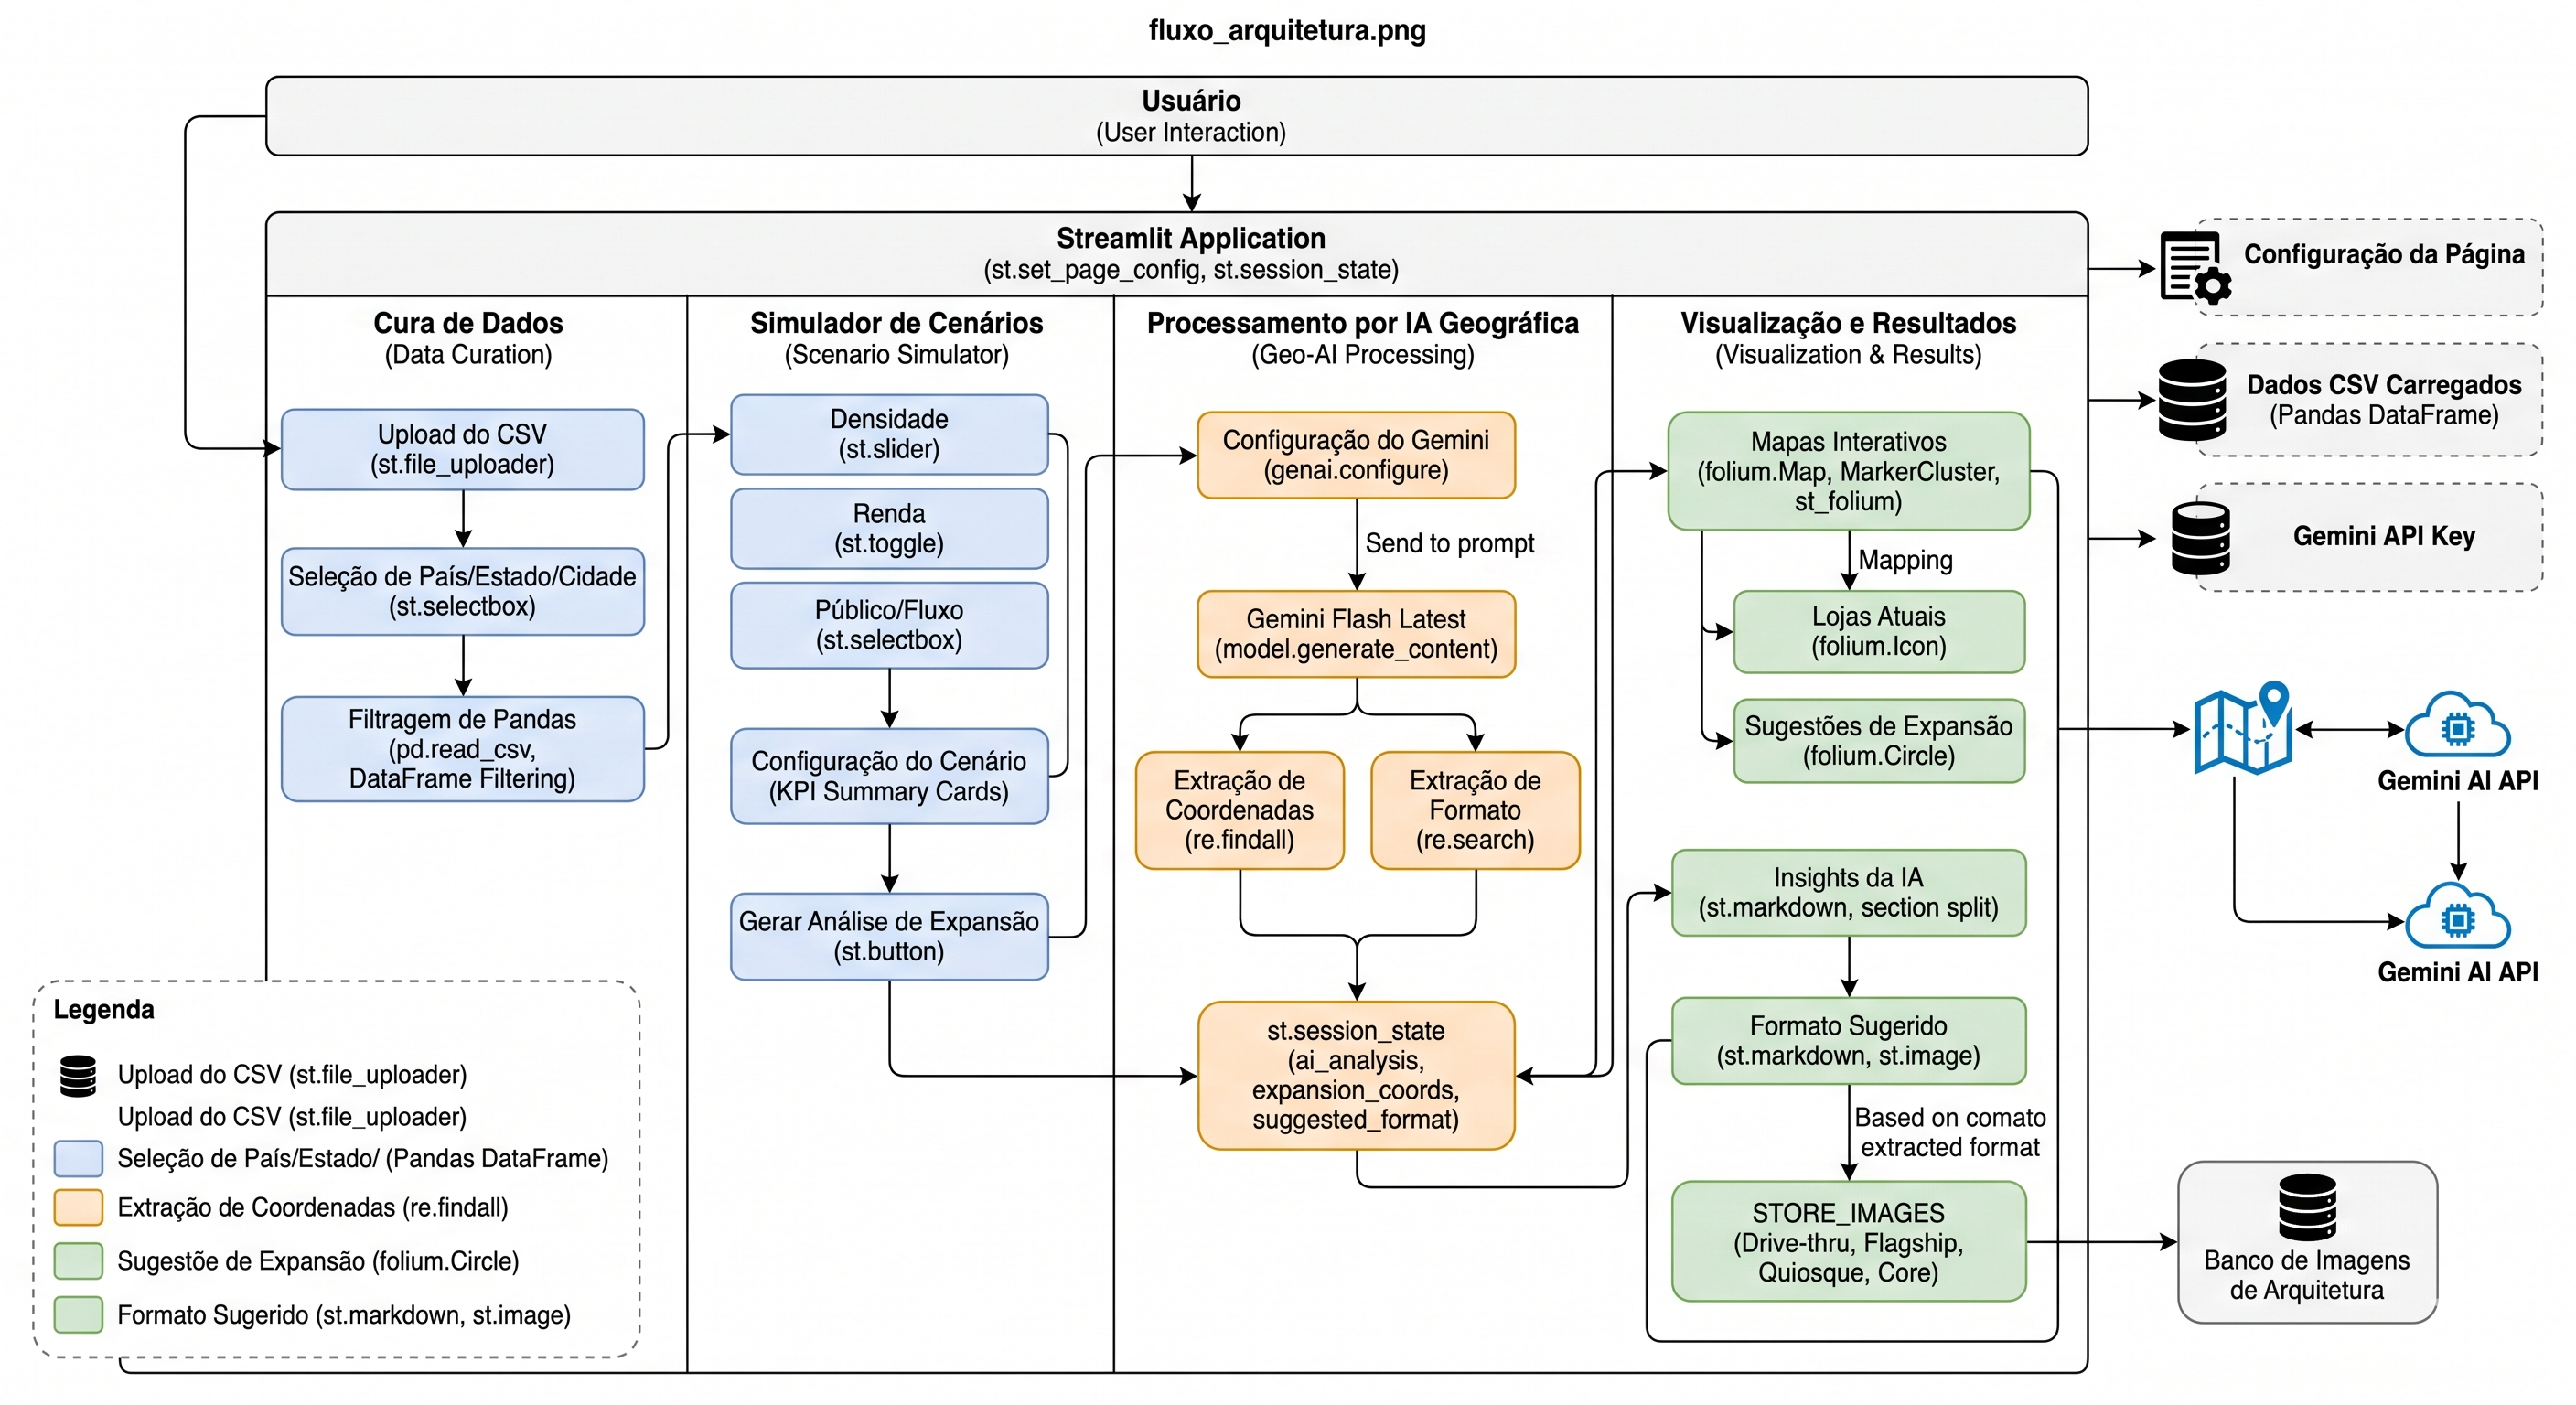
\includegraphics[width=0.8\textwidth]{fluxo-arquitetura.png}
    \vspace{0.2cm}
    \\\\\\
    \centering
    { \footnotesize \textbf{Fonte:} elaborada pela autora.\par}
\end{figure}

\begin{figure}[H]
    \captionsetup{justification=raggedright, singlelinecheck=false}
    \caption{Interface visual do sistema \textit{Retail Insights}. A imagem demonstra a disposição dos filtros geográficos e o simulador de cenários, permitindo ao usuário ajustar variáveis de densidade e renda em tempo real.}
    \centering
    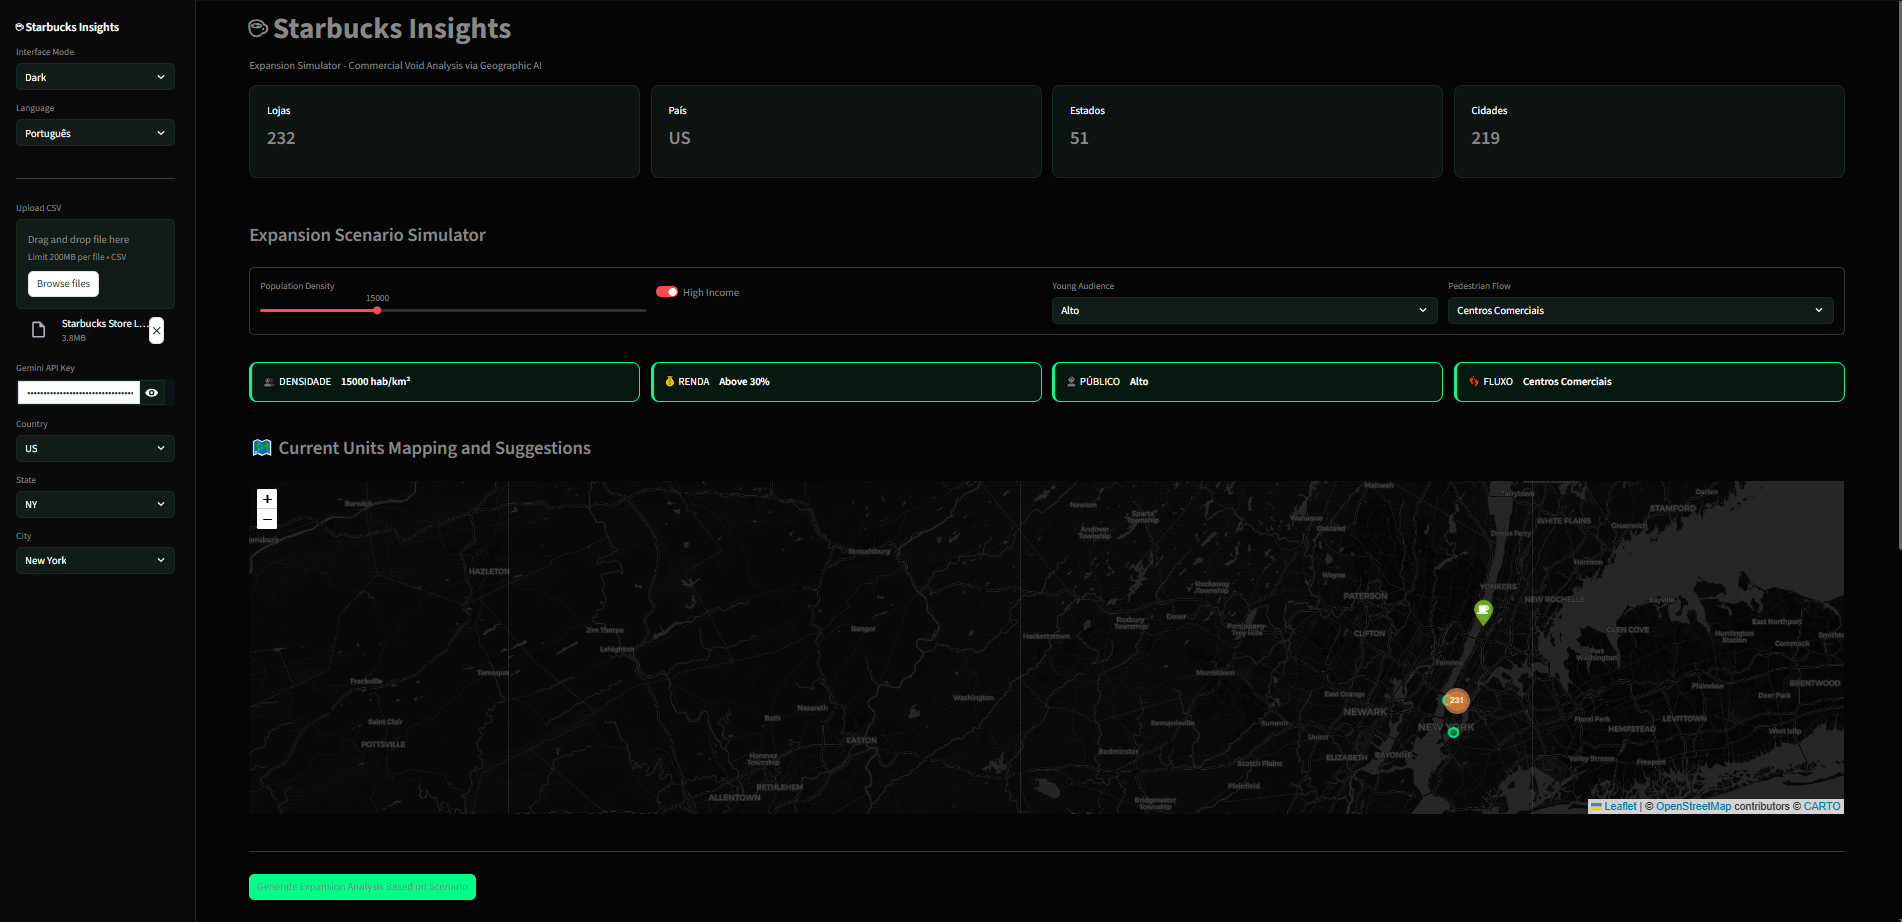
\includegraphics[width=0.9\textwidth]{Image.png}
    \vspace{0.2cm}
    \\\\\\
    \centering
    {\footnotesize \textbf{Fonte:} elaborada pela autora.\par}
\end{figure}

\begin{figure}[H]
    \captionsetup{justification=raggedright, singlelinecheck=false}
    \caption{Relatório de Análise de Expansão gerado pela IA. O painel exibe os \textit{insights} estratégicos produzidos pelo modelo \textit{Gemini}, justificando a escolha das localizações com base nos KPIs socioeconômicos definidos.}
    \centering
    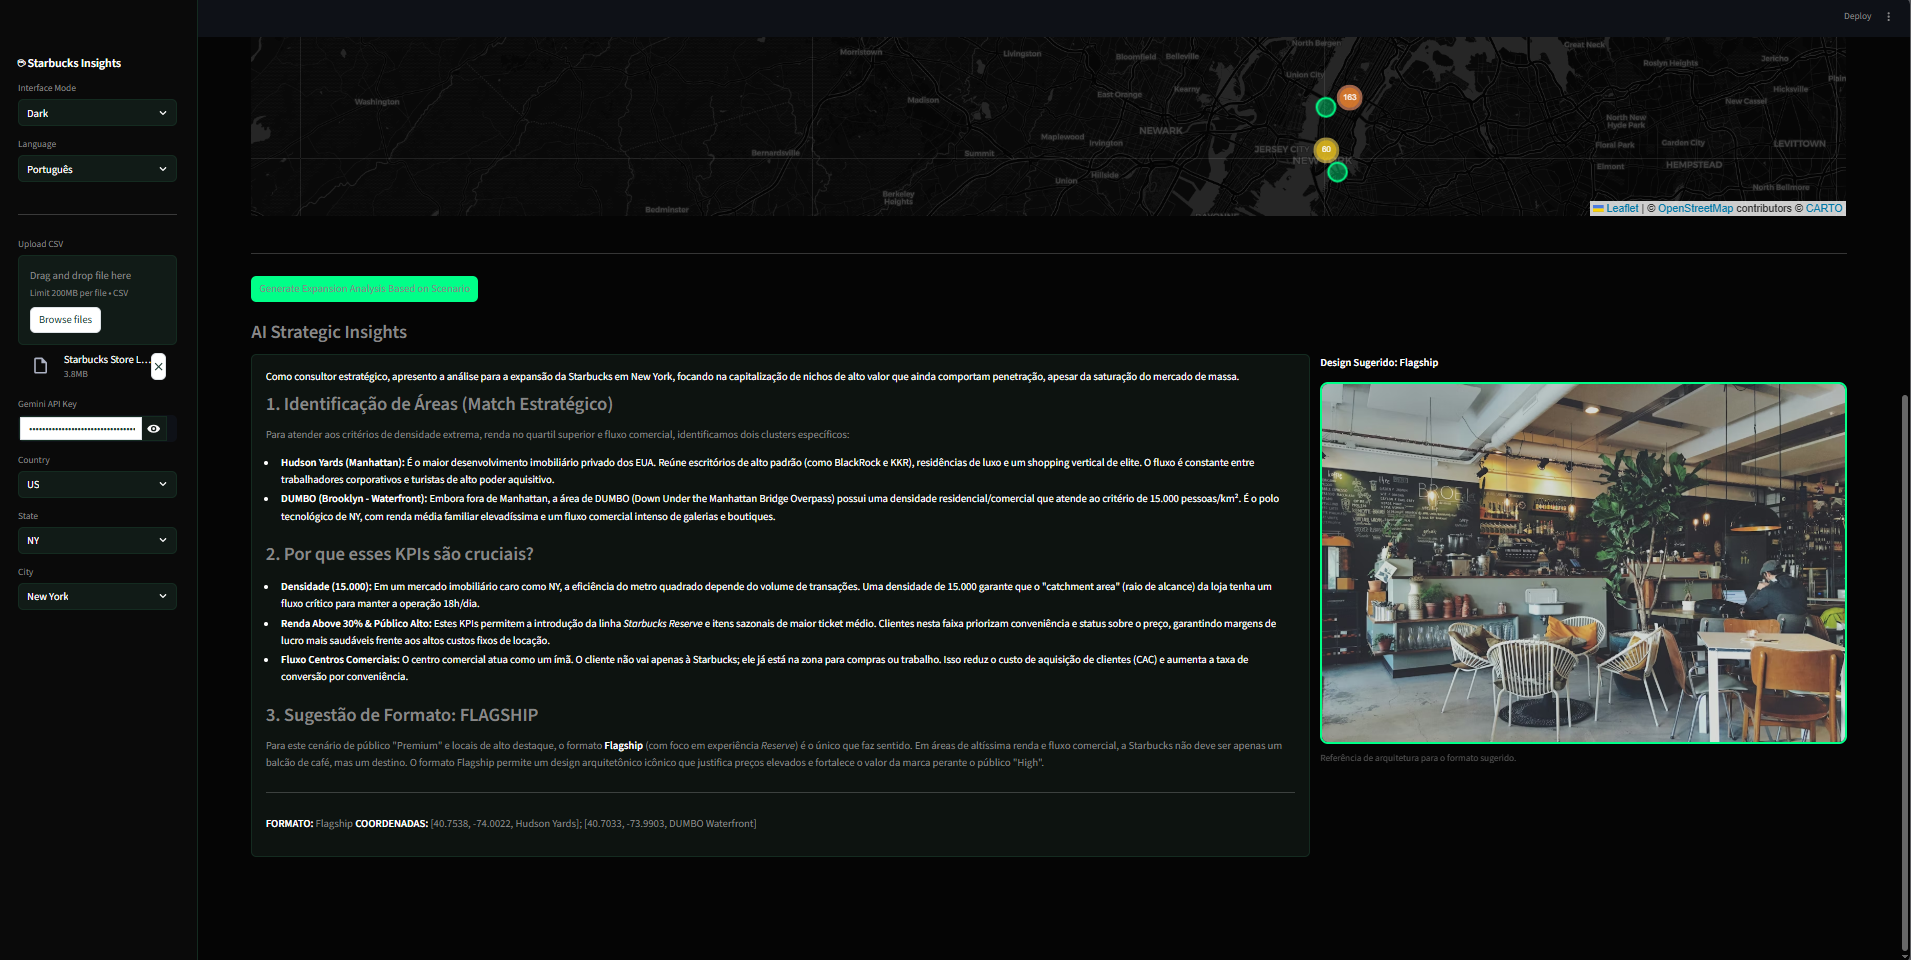
\includegraphics[width=0.9\textwidth]{image-2.png}
    \vspace{0.2cm}
    \\\\\\
    \centering
    {\footnotesize \textbf{Fonte:} elaborada pela autora.\par}
\end{figure}

A integração desses componentes resulta em uma ferramenta robusta para a escolha de pontos comerciais. O processo de expansão organizacional baseia-se em evidências de dados, conforme demonstrado no código-fonte disponível no apêndice.


\section{\esp Metodologia}


\subsection{\esp Etapas da pesquisa}

\begin{enumerate}
\item \textbf{Levantamento bibliográfico:} Buscamos trabalhos correlatos sobre IA e dados espaciais. Utilizamos a base IEEE Xplore com a \textit{string} de busca ("Artificial Intelligence") AND ("retail expansion"). O processo resultou em 12 artigos relevantes entre 2020 e 2025.

\item \textbf{Coleta de dados quantitativos:} Obtivemos a base geográfica global da rede \textit{Starbucks} referente a 2023, contendo \textbf{25.601 registros} distribuídos em \textbf{73 países}, \textbf{5.281 cidades} e \textbf{338 unidades federativas}. O arquivo inclui metadados cadastrais (marca, regime de operação, endereço, telefone, fuso horário) e coordenadas de latitude/longitude para plotagem no mapa. As variáveis socioeconômicas (densidade demográfica, renda, perfil etário e fluxo de pedestres) são parametrizadas dinamicamente pelo usuário via \textit{sliders} na interface, não armazenadas no \textit{CSV}.

\item \textbf{Criação da chave de \textit{API Key} do \textit{Gemini}:} criação de uma credencial no \href{https://aistudio.google.com/}{\textit{Google AI Studio}} para integração com o modelo \texttt{gemini-3.1-flash-lite}, selecionado pela maior cota gratuita de requisições diárias (500 \textit{RPD}).

\item \textbf{Configuração do banco de dados \textit{Supabase}:} criação das tabelas \texttt{lojas}, \texttt{respostas} e \texttt{store\_images}, com habilitação de \textit{Row Level Security} (RLS) e definição de políticas de leitura pública e escrita autenticada. Migração dos registros do arquivo \textit{CSV} para a tabela \texttt{lojas} e inserção das 20 referências arquitetônicas na tabela \texttt{store\_images}.

\item \textbf{Desenvolvimento da interface interativa:} Criamos o ambiente visual para exibir os resultados da IA. Implementamos a análise de cenários, permitindo ao usuário manipular \textit{cards} interativos para alterar os KPIs.

\item \textbf{Aplicação do estudo de caso:} Inserimos as variáveis da rede \textit{Starbucks} no sistema. Parametrizamos o modelo para testar hipóteses de densidade, renda, perfil jovem e fluxo de pedestres.

\item \textbf{Análise dos resultados:} Avaliamos de forma quantitativa e espacial as áreas indicadas pela IA. Verificamos a precisão da interface na adaptação aos cenários estipulados.
\end{enumerate}

O desenvolvimento experimental utilizou a linguagem Python e as bibliotecas \href{https://streamlit.io/}{\textit{Streamlit}}, \href{https://pandas.pydata.org/}{\textit{Pandas}}, \href{https://python-visualization.github.io/folium/}{\textit{Folium}}, \href{https://ai.google.dev/api/python/google/generativeai}{\textit{Google Generative AI}} e o cliente Python do \textit{Supabase}. Os dados persistentes no banco e as variáveis de cenário fornecidas pelo usuário passam pelo modelo \texttt{gemini-3.1-flash-lite} via \textit{API Key} para classificar as áreas de expansão. Validamos o sistema pela mensuração da precisão técnica ao sugerir localizações baseadas em evidências.


\subsection{\esp Classificação da pesquisa}
Em relação à sua natureza, este trabalho foi caracterizado como uma pesquisa aplicada, pois direciona o conhecimento científico para a solução de um problema prático específico: a otimização da expansão comercial por meio da tecnologia. Quanto à sua abordagem, trata-se de uma pesquisa quantitativa, lidando com o processamento de métricas numéricas e dados espaciais precisos. Do ponto de vista dos objetivos, a pesquisa foi classificada como descritiva, uma vez que busca descrever as características de determinadas regiões geográficas e o padrão de distribuição dos novos pontos comerciais.

No que tange aos procedimentos técnicos, foi utilizado o método experimental, evidenciado pelo desenvolvimento em Python, utilizando como base a \textit{API} \textit{Gemini}, teste e validação para a interface. Em conjunto, adota o formato de estudo de caso, focando na aplicação prática dessa ferramenta computacional na estratégia de expansão da rede Starbucks, permitindo uma análise em um cenário real de negócios.


Os dados de localização das lojas Starbucks utilizados nesta pesquisa foram obtidos via plataforma \textit{Kaggle}, representando o cenário global da rede em 2023 \cite{omarsobhy2023}. A coleta original foi realizada por meio de \textit{web scraping} que extraiu informações diretamente do portal corporativo da Starbucks. A extração automatizada consiste em uma técnica na qual um programa simula a navegação humana em páginas web, lê o código \textit{HyperText Markup Language} (HTML) e isola os elementos de interesse por meio de seletores estruturais.

No caso da base utilizada, o procedimento percorreu o diretório público de lojas do site da Starbucks e capturou recursivamente as páginas de cada unidade: país, estado, cidade, endereço, telefone, fuso horário e coordenadas geográficas. Os registros foram consolidados em um arquivo tabular. Essa abordagem disponibilizou um volume de dados que seria inviável coletar manualmente, permitindo à ferramenta operar sobre uma visão completa da pegada geográfica da rede e viabilizando a comparação entre regiões em escala global.

Após a captura, os dados passaram por processos de higienização e padronização para garantir a integridade das coordenadas geográficas e metadados. A estrutura resultante do arquivo .csv, detalhada no Quadro \ref{qua:estrutura_csv}, serviu de insumo para o processamento da Inteligência Artificial e a identificação de novos pontos comerciais.

\begin{quadro}[H]
    \captionsetup{justification=raggedright, singlelinecheck=false}
    \caption{Estrutura e metadados do arquivo .csv (Starbucks 2023)}
    \label{qua:estrutura_csv}
   \centering
\begin{tabular}{|l|p{5,2cm}|p{5,5cm}|}
\hline
\textbf{Campo (Coluna)} & \textbf{Descrição do Metadado} & \textbf{Tipo e Distribuição} \\ \hline
Brand & Marca vinculada à unidade. & \textit{String}. Starbucks (98,6\%), Teavana (1,4\%) \\ \hline
Store Number & Identificador único da loja. & \textit{String}. 25.599 valores únicos \\ \hline
Store Name & Nome de exibição da unidade. & \textit{String}. 22.708 valores únicos \\ \hline
Ownership Type & Regime de operação. & \textit{String}. Company Owned (46,6\%), Licensed (36,6\%), Joint Venture (15,5\%), Franchise (1,2\%) \\ \hline
Street Address & Endereço físico da unidade. & \textit{String}. 25.251 valores únicos \\ \hline
City & Cidade de localização. & \textit{String}. 5.281 valores distintos (Top: Seul, Nova York, Londres) \\ \hline
State/Province & Unidade federativa ou província. & \textit{String}. 338 valores distintos (Top: CA, TX, ENG) \\ \hline
Country & Código do país (ISO-3166 alfa-2). & \textit{String}. 73 países (US 53,2\%, CN 10,7\%, CA 5,7\%) \\ \hline
Postcode & Código postal / CEP. & \textit{String}. 6,0\% de valores ausentes \\ \hline
Phone Number & Contato telefônico da loja. & \textit{String}. 26,8\% de valores ausentes \\ \hline
Timezone & Fuso horário da unidade. & \textit{String}. 101 fusos distintos \\ \hline
Longitude & Coordenada geográfica (eixo X). & \textit{Decimal}. Faixa: $[-159,46; +176,92]$ \\ \hline
Latitude & Coordenada geográfica (eixo Y). & \textit{Decimal}. Faixa: $[-46,41; +64,85]$ \\ \hline
\end{tabular}

\vspace{0.1cm}
\centering
    {\footnotesize \textbf{Fonte:} adaptada de Kaggle (2023).}

\end{quadro}

\section{\esp Resultados} 

A plataforma \textit{Retail Insights} utiliza o modelo Gemini, via Google AI Studio, para processar dados geográficos e socioeconômicos. A ferramenta opera integrada ao arquivo \textit{CSV} da rede Starbucks. O motor de IA interpreta a distribuição das lojas atuais e gera visualizações espaciais. O sistema produz relatórios técnicos baseados em critérios de negócio inseridos em tempo real.

\subsection{\esp Processamento de KPIs e Círculos Demográficos}

A interface oferece um painel interativo. Nele, configuramos cenários prospectivos com quatro indicadores fundamentais. O modelo \textit{Gemini} analisa os dados e delimita círculos demográficos no mapa. Estes círculos indicam regiões propícias à expansão. A análise foca nos seguintes parâmetros:

\begin{enumerate}
    \item \textbf{Densidade populacional:} identifica áreas com alta concentração de habitantes.
    \item \textbf{Renda familiar:} prioriza regiões com renda 30\% superior à média nacional.
    \item \textbf{Público jovem:} define a presença deste perfil como variável binária.
    \item \textbf{Fluxo de pedestres:} prioriza zonas de alto tráfego para novos pontos.
\end{enumerate}

O mapa interativo plota as unidades existentes enquanto o painel lateral processa os comandos. Após o processamento, o \textit{Gemini} gera um relatório de \textit{insights} (Figura \ref{relatorio}). O documento justifica a escolha de cada bairro. Além disso, correlaciona a ausência de lojas com o potencial econômico detectado.

\begin{figure}[H]
    \captionsetup{justification=raggedright, singlelinecheck=false}
    \caption{Relatório de análise de expansão gerado pela IA. O painel detalha a viabilidade técnica das áreas sugeridas, cruzando densidade demográfica e renda para validar o formato de loja proposto.}
    \centering
    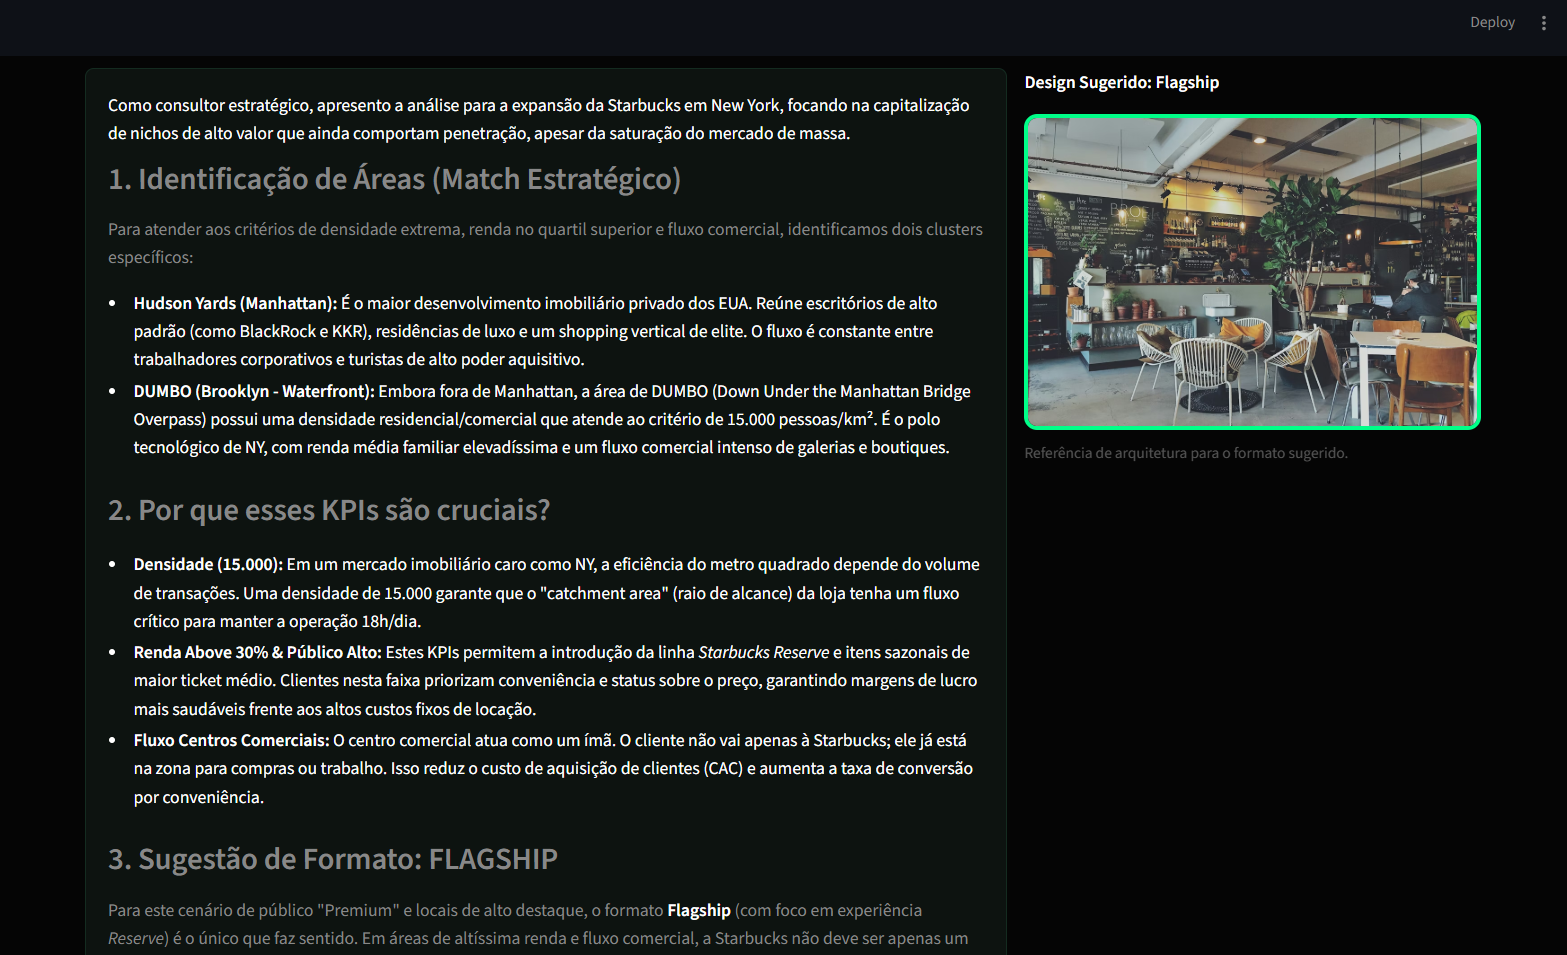
\includegraphics[width=0.9\textwidth]{relatorio-analise.png}
    \vspace{0.2cm}
\\\\\\    \label{relatorio}
    { \footnotesize \textbf{Fonte:} elaborada pela autora.\par}
\end{figure}

A Figura \ref{fig:mapa_unidades} ilustra a distribuição espacial das unidades. Utilizamos uma escala cromática para representar a saturação comercial. O marcador verde sinaliza baixa densidade de lojas. O marcador amarelo indica densidade média. O marcador vermelho aponta alta concentração de estabelecimentos. Os círculos verdes transparentes delimitam as regiões sugeridas para expansão. Tais sugestões baseiam-se nos KPIs socioeconômicos selecionados pelo analista.

\subsection{\esp Estudo de Caso: Cidade de New York, NY}

Para demonstrar objetivamente a aplicação da ferramenta, executamos um cenário real sobre a cidade de \textbf{New York, NY}. A entrada fornecida ao sistema foi o recorte da tabela \texttt{lojas} (base de dados \textit{CSV} Starbucks 2023, migrada para o \textit{Supabase}) filtrado para essa localidade -- uma das cidades com maior concentração de unidades da rede no mundo, conforme detalhado no Quadro \ref{qua:estrutura_csv}. No simulador, fixamos os seguintes parâmetros: densidade demográfica superior a 15.000 hab/km\textsuperscript{2}, renda familiar acima de US\$ 100 mil/ano (acima de 30\% da média nacional), forte fluxo de centros comerciais e distritos de alto consumo.

O modelo \texttt{gemini-3.1-flash-lite} processou o cenário e devolveu dois pontos de expansão acompanhados de coordenadas geográficas e justificativa textual. Em ambos os casos, a IA recomendou o formato \textbf{\textit{core}} (loja compacta, otimizada para espaço e custo-eficiência em zonas de aluguel premium), com foco em visibilidade de marca, atendimento ágil, conveniência e alta rotatividade -- características adequadas ao mercado imobiliário de New York. As localizações sugeridas foram:

\begin{itemize}
    \item \textbf{Upper West Side (Broadway \& 72nd St)} -- coordenadas aproximadas \texttt{[40,7784; -73,9820]} -- formato sugerido: \textit{core}; justificativa: região com uma das maiores densidades de residentes com renda superior a 30\% acima da média da cidade, fluxo constante de transeuntes em direção às estações de metrô e varejo consolidado, garantindo aderência ao público-alvo.
    \item \textbf{Williamsburg (Bedford Ave, Brooklyn)} -- coordenadas aproximadas \texttt{[40,7142; -73,9628]} -- formato sugerido: \textit{core}; justificativa: consolidou-se como polo de maior poder aquisitivo jovem de New York, com densidade crescente e fluxo intenso de centros comerciais de rua que atraem tanto residentes quanto turistas de alto padrão.
\end{itemize}

Vale destacar, ainda, que a ferramenta evita sugerir áreas já saturadas. Ao avaliar o entorno de \textbf{Times Square} (Manhattan), o sistema não recomendou a abertura de novas unidades: a região apresenta concentração elevada de lojas Starbucks já existentes (saturação alta no mapa cromático), o que reduziria o potencial de retorno de um novo ponto. Esse comportamento confirma que a IA respeita o critério de saturação comercial e concentra recomendações em zonas de vazio de mercado.

A Figura \ref{fig:mapa_unidades} apresenta o mapa resultante, com os círculos verdes transparentes delimitando as regiões sugeridas. Ao cruzar as sugestões com o mapa de saturação comercial (escala verde $\rightarrow$ vermelho), constata-se que ambas as áreas correspondem a zonas de saturação limitada, ainda que inseridas em distritos de alto consumo -- o que corrobora a hipótese de vazios comerciais identificados pela ferramenta. Este exemplo concreto evidencia o fluxo completo da solução: \textbf{entrada} (recorte da base Starbucks), \textbf{processamento} (motor de IA com KPIs parametrizados) e \textbf{saída} (coordenadas geográficas, justificativa textual e formato de loja sugerido).

\begin{figure}[H]
    \captionsetup{justification=raggedright, singlelinecheck=false}
    \caption{Mapa interativo de densidade e sugestões de expansão. A escala de cores (verde a vermelho) indica a concentração de lojas atuais. Os círculos transparentes marcam os novos pontos de alto potencial sugeridos pela IA.}
    \label{fig:mapa_unidades}
    \centering
    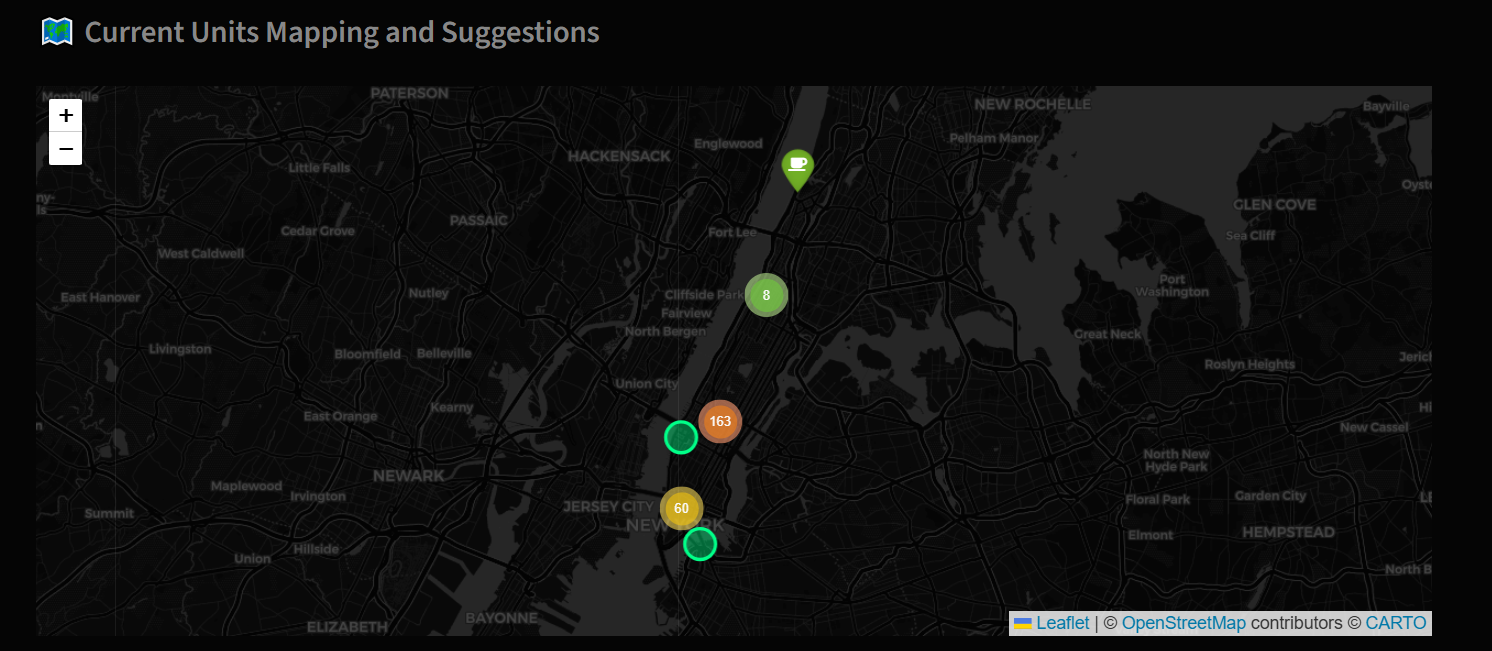
\includegraphics[width=0.9\textwidth]{mapa.png}
    \vspace{0.2cm}
    \\\\\\
    { \footnotesize \textbf{Fonte:} elaborada pela autora.\par}
\end{figure}

\subsection{\esp Comparação com a Análise Manual Tradicional}

Para evidenciar a contribuição da ferramenta, é fundamental contrastá-la com o processo manual ainda predominante em redes varejistas. Na análise tradicional, o Analista de Expansão precisa coletar, em fontes dispersas, dados demográficos (Censo IBGE), mapas de concorrência (Google Maps), relatórios de fluxo de pedestres (estudos encomendados a empresas especializadas) e indicadores socioeconômicos de renda. Em seguida, ele consolida essas informações em planilhas eletrônicas, aplica filtros manuais e fundamenta a recomendação de localização majoritariamente em sua experiência pessoal e em visitas \textit{in loco}. Esse fluxo consome, tipicamente, de alguns dias a algumas semanas por região avaliada e está sujeito à subjetividade do analista, à baixa rastreabilidade dos critérios e à dificuldade de replicar o estudo em diferentes cidades \cite{mallela2024, okorie2024}.

A plataforma \textit{Retail Insights}, por sua vez, automatiza esse fluxo. O cruzamento de KPIs (densidade, renda, perfil etário e fluxo de pedestres) com a distribuição das unidades existentes é realizado em segundos pelo modelo \textit{Gemini}, que devolve coordenadas geográficas precisas acompanhadas de justificativa textual e do formato de loja sugerido. O Quadro \ref{qua:comparativo} sintetiza essa comparação.

\begin{quadro}[H]
    \centering
    \captionsetup{justification=raggedright, singlelinecheck=false}
    \caption{Comparativo entre análise manual tradicional e a ferramenta proposta.}
    \label{qua:comparativo}
    \begin{tabular}{|p{4,0cm}|p{5,0cm}|p{5,0cm}|}
    \hline
    \textbf{Critério} & \textbf{Análise Manual Tradicional} & \textbf{Retail Insights (proposta)} \\ \hline
    Fonte dos dados & Dispersa (IBGE, Google, relatórios pagos) & Centralizada no \textit{Supabase}, integrada ao \textit{CSV} Starbucks \\ \hline
    Tempo de análise & Dias a semanas por região & Segundos por cenário parametrizado \\ \hline
    Subjetividade & Elevada (depende da experiência do analista) & Reduzida (critérios explícitos e replicáveis) \\ \hline
    Rastreabilidade & Limitada (planilhas locais) & Total (relatório técnico gerado pela IA) \\ \hline
    Visualização & Mapas estáticos & Mapa interativo com escala cromática e círculos de potencial \\ \hline
    Escalabilidade & Baixa (esforço cresce linearmente) & Alta (mesmo fluxo para qualquer cidade do \textit{dataset}) \\ \hline
    \end{tabular}
    \vspace{0.1cm}
    \centering
    {\footnotesize \textbf{Fonte:} elaborada pela autora.\par}
\end{quadro}

Cabe destacar que a ferramenta não substitui integralmente o julgamento humano; em vez disso, atua como uma camada de suporte à decisão que padroniza o conjunto mínimo de evidências e libera o analista para avaliar aspectos qualitativos (tamanho do ponto comercial, custo de arrendamento, condições de acesso), atividade em que a intuição humana ainda supera a IA.

\subsection{\esp Integração com Gemini}

O Algoritmo \ref{alg:codigo_python} detalha a lógica de conexão entre a linguagem \href{https://www.python.org/}{\textit{Python}} e a \textit{API} do \textit{Gemini}. O código lê o arquivo extraído do Kaggle e submete as variáveis de interesse ao modelo de linguagem para processamento estratégico.

\begin{lstlisting}[language=Python, captionpos=t, caption={Trecho principal do código de integração com a IA.}, label={alg:codigo_python}]
# O sistema utiliza a API Key do Google AI Studio
import google.generativeai as genai

# Funcao cacheada para evitar chamadas duplicadas a API
@st.cache_data(show_spinner=False)
def obter_analise_ia(api_key, cidade, num_lojas, densidade, renda, publico, fluxo):
    genai.configure(api_key=api_key)
    model = genai.GenerativeModel('gemini-3.1-flash-lite')
    # O prompt restringe a analise a cidade selecionada e exige formato estruturado
    prompt = (f"Consultor estrategico: analise expansao na cidade de {cidade}. "
              f"Lojas atuais: {num_lojas}. Cenario: Densidade {densidade}, "
              f"Renda {renda}, Publico {publico}, Fluxo {fluxo}. "
              f"Identifique 2 areas reais. Sugira formato: Drive-thru, Flagship, "
              f"Quiosque ou Core. Finalize com: FORMATO: [Nome] e "
              f"COORDENADAS: [LAT, LON, NOME]; [LAT, LON, NOME]")
    response = model.generate_content(prompt)
    return response.text
\end{lstlisting}

\vspace{0.1cm}
{\centering \footnotesize \textbf{Fonte:} elaborada pela autora.\par}

\subsection{\esp Avaliação de Experiência do Usuário (Escala Likert)}

Integramos um formulário de avaliação baseado na escala \textit{Likert} após a geração do relatório estratégico. Mensuramos a satisfação do usuário por meio de cinco níveis visuais (\textit{emojis}). O formulário (Figura \ref{fig:likert}) avalia intuitividade, clareza visual e desempenho do sistema para auxiliar no processo de melhoria contínua da experiência do usuário (\textit{UX}).

\subsubsection{\esp Construção do questionário}

O questionário foi estruturado em quatro perguntas de múltipla escolha, utilizando escala \textit{Likert} de 5 pontos representada visualmente por \textit{emojis} (1 -- Péssimo; 2 -- Ruim; 3 -- Médio; 4 -- Bom; 5 -- Excelente). As perguntas, aplicadas após o respondente interagir com o simulador e visualizar o relatório gerado pela IA, buscaram captar percepções sobre dimensões complementares da ferramenta: (Q1) intuitividade da interface (``A interface é intuitiva?''); (Q2) contribuição do \textit{design} visual (``O \textit{design} visual ajudou?''); (Q3) relevância dos \textit{insights} produzidos pela IA (``A IA foi relevante?''); e (Q4) utilidade da visualização geoespacial (``O mapa ajudou?''). A opção por quatro perguntas curtas teve como finalidade reduzir o esforço de resposta e ampliar a taxa de adesão, ao mesmo tempo em que permitiu separar o julgamento sobre a camada de interação (Q1 e Q2) do julgamento sobre as saídas analíticas da ferramenta (Q3 e Q4). A redação foi testada preliminarmente com dois colegas do curso de Sistemas de Informação e ajustada quanto à clareza antes da aplicação.

\subsubsection{\esp Amostra e aplicação}

O link público da ferramenta, acompanhado de uma breve descrição do objetivo do estudo e do termo de consentimento, foi encaminhado para \textbf{100 pessoas}. Os participantes foram selecionados por conveniência, com os seguintes critérios: (a) serem profissionais, estudantes ou pesquisadores com vínculo direto ou indireto com o varejo, marketing, tecnologia da informação ou análise de dados (a amostra efetiva incluiu analistas de dados, desenvolvedores de software, engenheiros de IA, professores e estudantes); (b) terem familiaridade mínima com interfaces web; e (c) terem acessado a ferramenta e visualizado pelo menos um relatório gerado pela IA. A aplicação ocorreu ao longo de \textbf{3 semanas}, ao final das quais \textbf{21 respondentes} haviam preenchido efetivamente o formulário -- taxa de resposta de 21\%, compatível com surveys online sem incentivo financeiro.

A Tabela \ref{tab:likert} apresenta as médias obtidas em cada pergunta. Observa-se que as dimensões relacionadas às \textbf{saídas analíticas} da ferramenta obtiveram avaliação levemente superior (\textbf{3,90} tanto para a relevância dos \textit{insights} da IA quanto para a utilidade do mapa). Já as dimensões ligadas à \textbf{camada de interação} receberam avaliação mais contida (\textbf{3,19} para intuitividade da interface e \textbf{3,76} para o \textit{design} visual). A média global foi de \textbf{3,69} em escala de 1 a 5.

Esse comportamento sugere que a ferramenta entrega valor por meio de seus resultados -- os \textit{insights} e a visualização geoespacial --, mas indica espaço para evolução da usabilidade. As ressalvas provavelmente estão associadas à latência da \textit{API} do \textit{Gemini} e à curva de aprendizado dos filtros regionais. Nenhuma pergunta apresentou média abaixo do nível ``Médio'' (3), o que indica recepção global positiva, ainda que não uniforme entre as dimensões.

\begin{table}[H]
    \centering
    \captionsetup{justification=raggedright, singlelinecheck=false}
    \caption{Médias obtidas no questionário \textit{Likert} por dimensão avaliada.}
    \label{tab:likert}
    \begin{tabular}{|c|p{7,5cm}|c|c|}
    \hline
    \textbf{Pergunta} & \textbf{Dimensão avaliada} & \textbf{Média (1--5)} & \textbf{Interpretação} \\ \hline
    Q1 & Intuitividade da interface & 3,19 & Médio \\ \hline
    Q2 & Contribuição do \textit{design} visual & 3,76 & Bom \\ \hline
    Q3 & Relevância dos \textit{insights} da IA & 3,90 & Bom \\ \hline
    Q4 & Utilidade do mapa interativo & 3,90 & Bom \\ \hline
    \multicolumn{2}{|r|}{\textbf{Média global}} & \textbf{3,69} & \textbf{Bom} \\ \hline
    \end{tabular}
    \vspace{0,1cm}
    \centering
    {\footnotesize \textbf{Fonte:} elaborada pela autora (n=21).\par}
\end{table}

Reconhecemos que o tamanho reduzido da amostra ($n=21$) constitui uma limitação importante do estudo, impedindo generalizações estatísticas e exigindo cautela na interpretação dos resultados; recomenda-se, em trabalhos futuros, ampliar a amostra e diversificar o perfil dos respondentes.

Armazenamos as avaliações coletadas na plataforma \href{https://supabase.com/}{\textit{Supabase}}, na tabela \texttt{respostas}, cuja coluna \texttt{contato} foi convertida para o tipo \texttt{text} para aceitar tanto telefone quanto e-mail. O fluxo de \textit{feedback} foi refinado: após a submissão, a interface exibe um \textit{card} persistente de confirmação (``Avaliação enviada com sucesso!'') em vez de uma mensagem efêmera, melhorando a clareza da UX. Além das avaliações, o \textit{Supabase} hospeda as tabelas \texttt{lojas} (CSV Starbucks migrado) e \texttt{store\_images} (20 referências arquitetônicas categorizadas em \textit{drive-thru}, \textit{flagship}, \textit{quiosque} e \textit{core}). Realizamos testes iniciais com volume limitado de registros. A limitação ocorreu devido a instabilidades na cota de \textit{tokens} da \textit{API} do \textit{Gemini} durante a fase experimental. Contudo, os registros validam a comunicação entre a interface e o servidor \textit{backend}. A Figura \ref{fig:supabase} demonstra a persistência dessas informações no banco de dados.

\begin{figure}[H]
    \captionsetup{justification=raggedright, singlelinecheck=false}
    \caption{Interface do formulário de avaliação \textit{Likert}. O sistema coleta percepções qualitativas sobre a utilidade da ferramenta e a precisão das análises geradas.}
    \label{fig:likert}
    \centering
    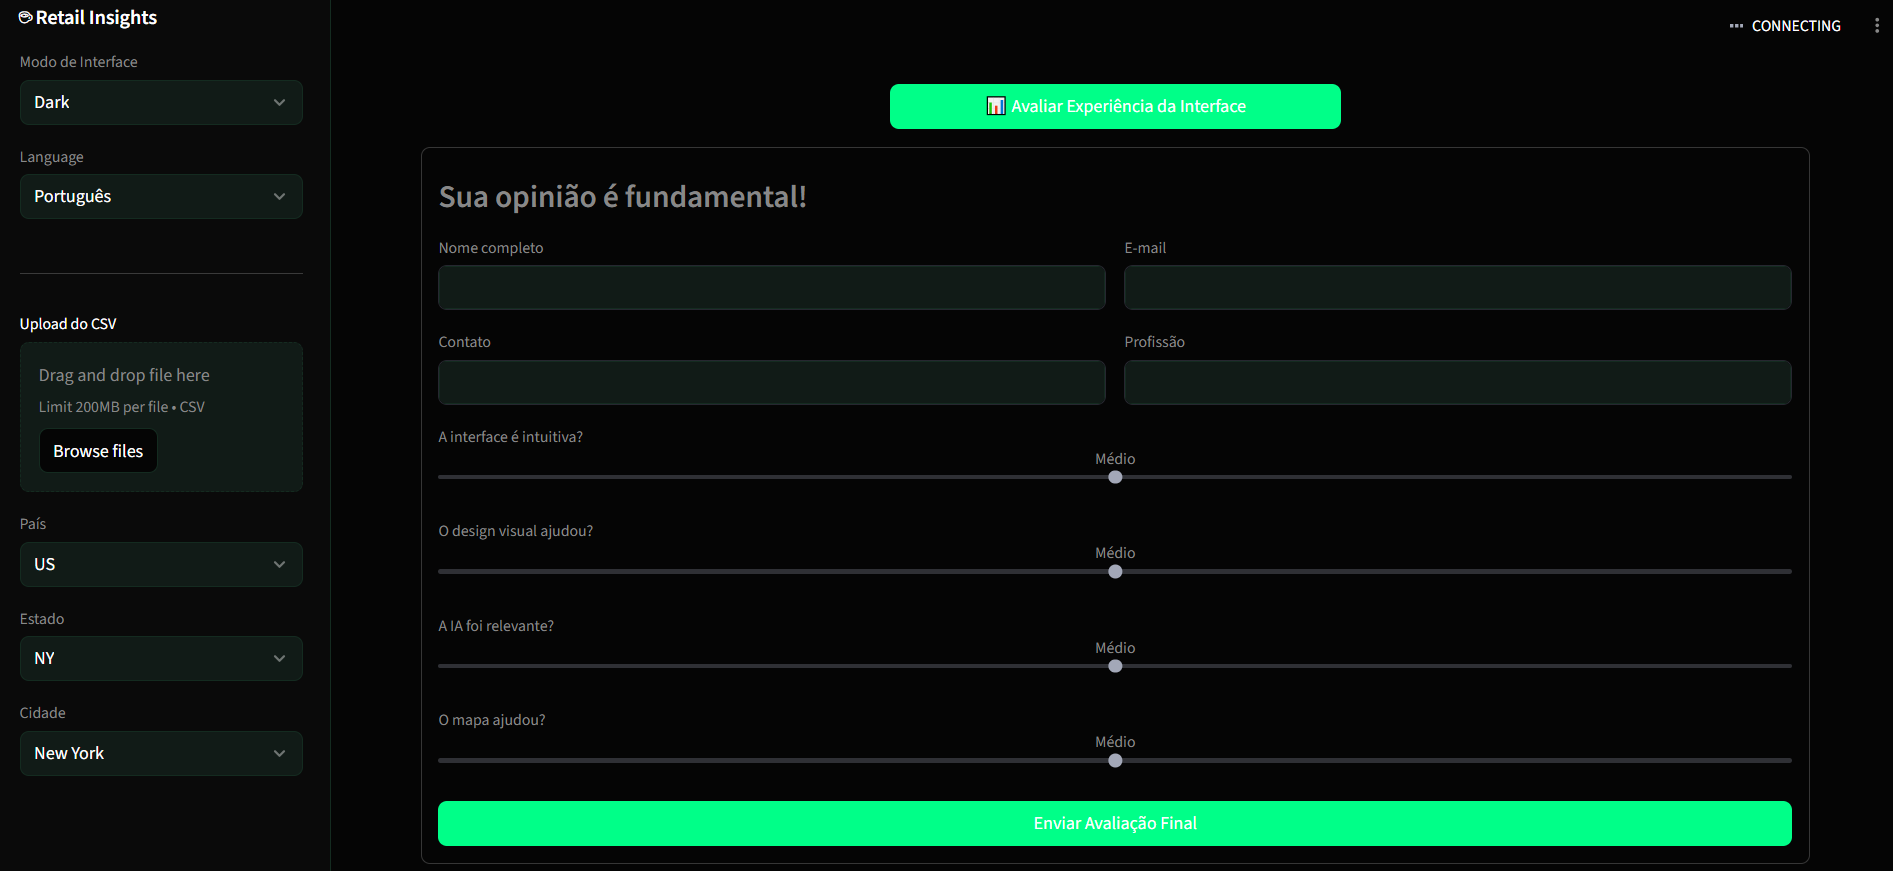
\includegraphics[width=0.9\textwidth]{formulario.png}
    \vspace{0.2cm}
    \\\\\\
    { \footnotesize \textbf{Fonte:} elaborada pela autora.\par}
\end{figure}

\begin{figure}[H]
    \captionsetup{justification=raggedright, singlelinecheck=false}
    \caption{Visualização das respostas no painel do \textit{Supabase}. A imagem confirma o fluxo completo de dados, desde a submissão do usuário até o armazenamento persistente no banco de dados.}
    \label{fig:supabase}
    \centering
    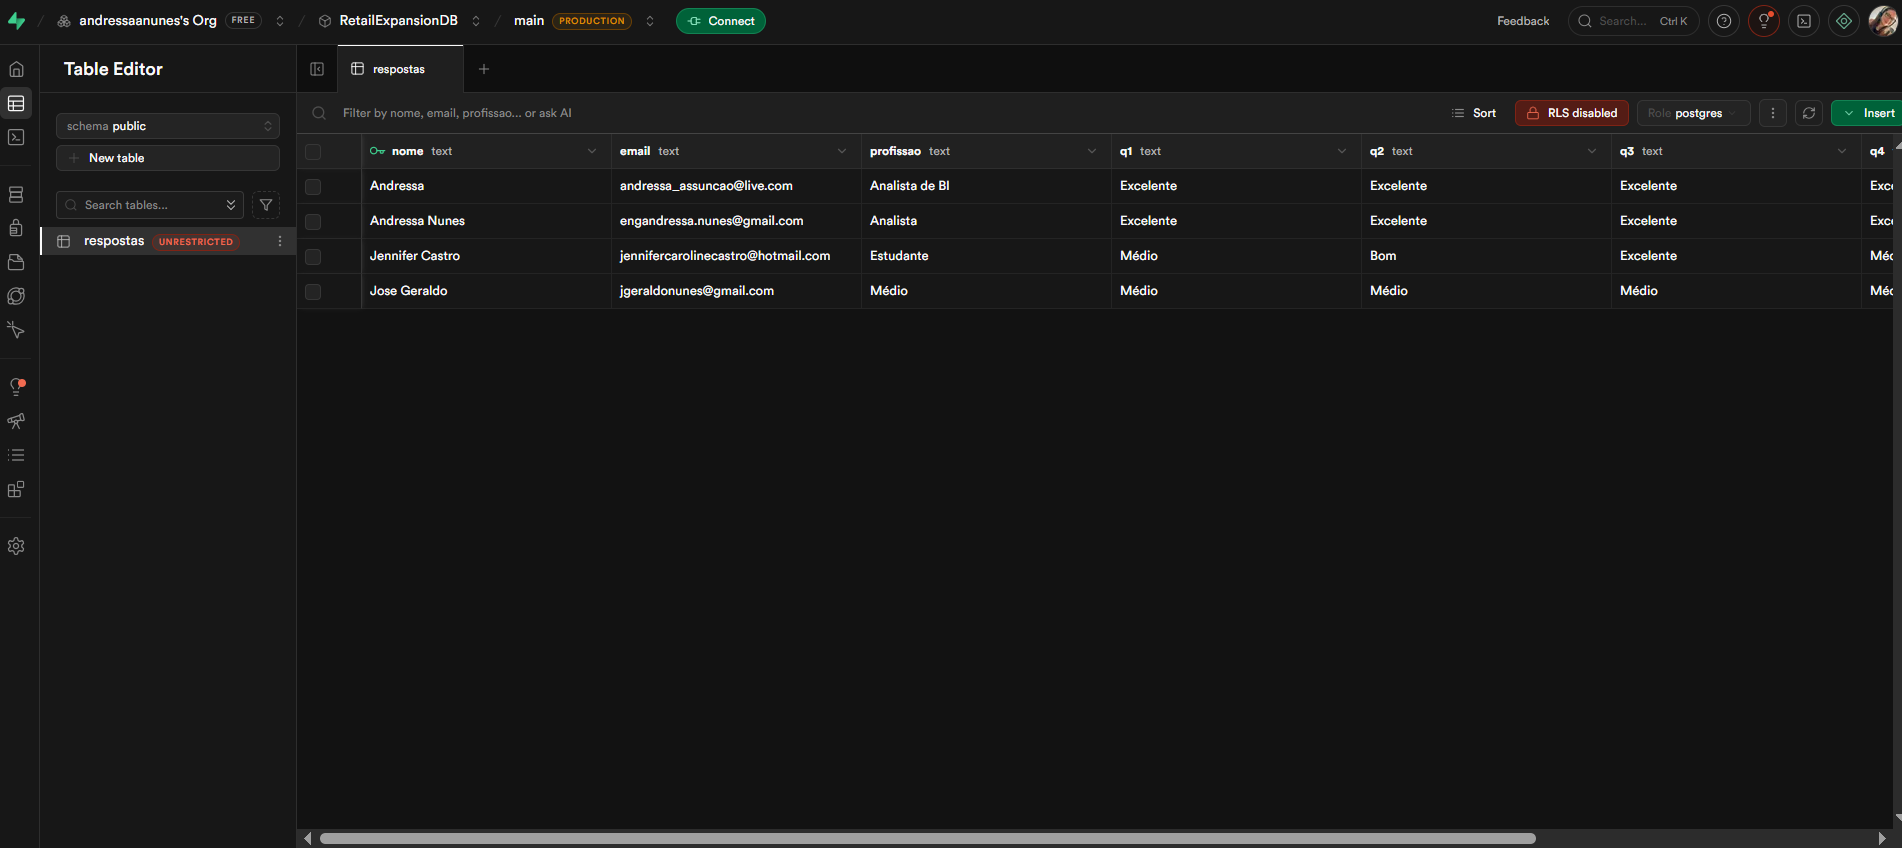
\includegraphics[width=0.9\textwidth]{supabase.png}
    \vspace{0.2cm}
    
    { \footnotesize \textbf{Fonte:} elaborada pela autora.\par}
\end{figure}
\section{\esp Conclusão}

Este trabalho apresenta o desenvolvimento da plataforma \textit{Retail Insights} para a análise geoestratégica de expansão varejista. O objetivo principal é alcançado por meio da integração entre a linguagem \textit{Python} e a \textit{API} do modelo \textit{Gemini}. Os resultados do estudo de caso demonstram que a ferramenta identifica vazios comerciais ao cruzar variáveis socioeconômicas e geográficas: as áreas sugeridas pela IA correspondem, de forma consistente, a zonas de baixa saturação comercial no mapa, o que valida a premissa de que o sistema localiza regiões com potencial de expansão. Contudo, é importante ressaltar que a ``precisão'' aqui mencionada refere-se à coerência entre os critérios parametrizados e as coordenadas devolvidas, e não a uma validação estatística formal contra o desempenho real de lojas abertas nessas localidades -- aspecto que permanece como limitação do estudo e recomenda avaliação futura. A aplicação no estudo de caso da rede \textit{Starbucks} valida a funcionalidade do sistema e viabiliza a prospecção de novos pontos comerciais baseada em evidências.

A discussão dos resultados indica que a solução supera modelos analíticos tradicionais ao reduzir a subjetividade do analista. A interface visual, por meio de uma escala cromática de densidade e círculos de expansão, facilita a interpretação de grandes volumes de dados espaciais. Uma vantagem central é a automação de relatórios estratégicos que justificam a viabilidade de cada localidade sugerida. No entanto, o sistema apresenta limitações: o desempenho das análises depende diretamente da qualidade e da atualização dos dados hospedados no banco \textit{Supabase} (com \textit{fallback} automático para o arquivo \textit{CSV} local), e a latência na geração de \textit{insights} varia conforme a estabilidade da conexão com os servidores da \textit{API} do \textit{Gemini}.

A principal contribuição desta pesquisa é a criação de uma metodologia para suporte à decisão em \textit{Business Intelligence} (BI). O trabalho entrega uma ferramenta funcional que converte indicadores estratégicos em saídas automatizadas. O uso de Inteligência Artificial Generativa para a identificação de novos pontos comerciais democratiza o acesso a análises complexas, antes restritas a consultorias especializadas. Dessa forma, a plataforma mitiga riscos financeiros e sustenta a expansão organizacional no mercado físico.

Como sugestão de trabalhos futuros, recomenda-se integrar dados de fluxo de pedestres em tempo real por meio de sensores de \textit{Internet of Things} (IoT). Além disso, sugere-se implementar a análise automatizada de concorrência direta para refinar as sugestões de localização. Recomendam-se, ainda, estudos posteriores para avaliar a aplicação desta interface em outros segmentos do varejo e do setor de serviços, a fim de testar a adaptabilidade do modelo lógico em diferentes contextos de mercado.

\endinput

%%%%%%%%%%%%%%%%%%%%%%%%%%%%%%%%%%%
%% FIM DO TEXTO
%%%%%%%%%%%%%%%%%%%%%%%%%%%%%%%%%%%

% \selectlanguage{brazil}
%%%%%%%%%%%%%%%%%%%%%%%%%%%%%%%%%%%
%% Inicio bibliografia
%%%%%%%%%%%%%%%%%%%%%%%%%%%%%%%%%%%

 \newpage
\singlespace{
\renewcommand\refname{REFERÊNCIAS}
\bibliography{bibliografia}
}

%Inclusão do arquivo abntex2-alf.bst como solução para adequação à ABNT NBR 10520:2023 quanto às citações, que não são mais em caixa-alta
\bibliographystyle{abntex2-alf.bst}
\include{apendices}
\end{document}